\begin{frame}{Problem: Over-fitting in a Neural Network}
	\begin{itemize}
		\item Why does over-fitting happen in a Neural network?
		\begin{itemize}
			\item too many free parameters
		\end{itemize}
	\end{itemize}
    \begin{figure}[H]
        \centering
        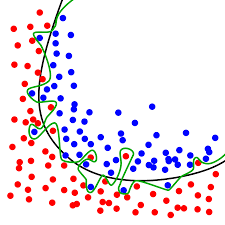
\includegraphics[width=0.4\textwidth]{Figs/section_4/overfitting.png}
        \caption{Over-fitting in a Neural Network \href{https://en.wikipedia.org/wiki/Overfitting}{source}}
    \end{figure}
\end{frame}

\begin{frame}{Solution 1: L1/L2 regularization}
    \begin{itemize}
        \item just like a classic regularizer
        \item sum the regularizer term for every layer weight
    \end{itemize}
    \vspace{0.2\textheight}
    \begin{equation*}
        \mathlarger{\mathlarger{\mathlarger{
        L = \frac{1}{N} \sum_{i=1}^{N} L(\phi(x_i), y_i) + \lambda \sum_{i,j,k} R(W_{j,k}^{(i)})
        }}}
    \end{equation*}
\end{frame}
\begin{frame}{Solution 1: L1/L2 regularization}
    \begin{itemize}
        \item L1/L2 regularizer functions (review)
    \end{itemize}
    \vspace{0.1\textheight}
    \begin{equation*}
        \mathlarger{\mathlarger{\mathlarger{
            L1: R(w) = \vert w\vert
        }}}
    \end{equation*}
    \begin{equation*}
        \mathlarger{\mathlarger{\mathlarger{
            L2: R(w) = w^2
        }}}
    \end{equation*}
    \begin{itemize}
        \item you can also combine the two different regularizers (Elastic net)
    \end{itemize}
    \vspace{0.1\textheight}
    \begin{equation*}
        \mathlarger{\mathlarger{\mathlarger{
        R(w) = \beta w^2 + \vert w\vert
        }}}
    \end{equation*}
\end{frame}

\begin{frame}{Solution 2: Early Stopping}
    \begin{itemize}
        \item Stop learning when the validation error is Minimum
    \end{itemize}
    \begin{figure}
	\centering
	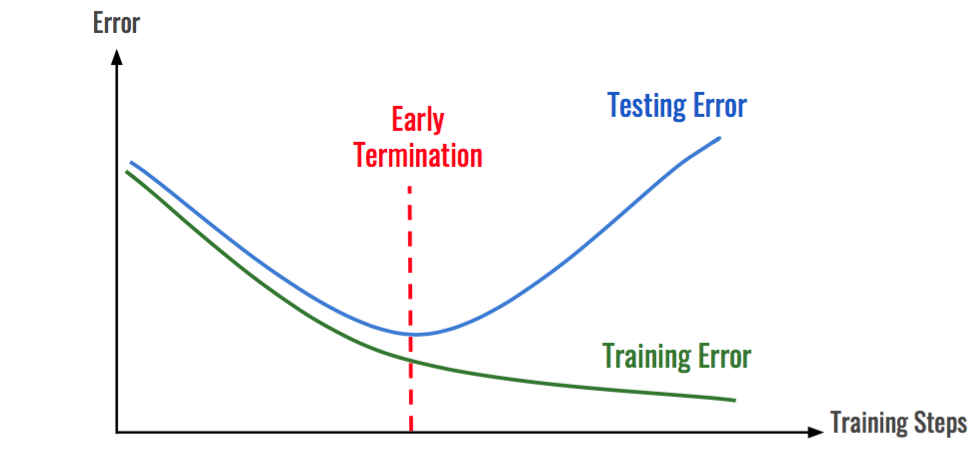
\includegraphics[width=0.8\textwidth]{Figs/Early Stopping.png}
	\caption{Early-Stopping diagram\href{https://medium.com/analytics-v7idhya/early-stopping-with-pytorch-to-restrain-your-model-from-overfitting-dce6de4081c5}{source}}
    \end{figure}
\end{frame}

\begin{frame}{Solution 3: Dropout}
	\begin{block}{Training}
		\begin{itemize}
			\item at each iteration, every neuron has a probability $P$ of being dropped out
			\begin{itemize}
				\item meaning it will be ignored
			\end{itemize}
			\item $P :=$ dropout rate
		\end{itemize}
		
		\begin{figure}[H]
			\centering
			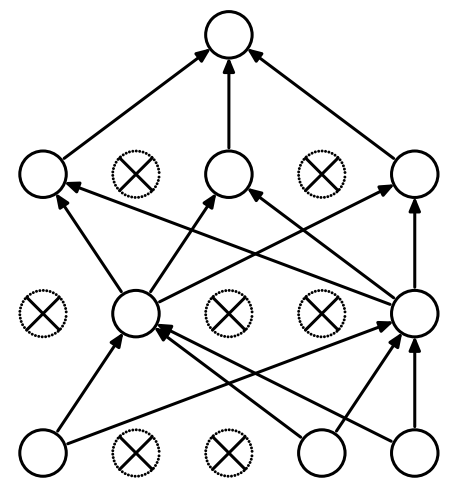
\includegraphics[height=0.4\textheight]{Figs/Dropout-after.png}
			\caption{Behavior of dropout at training time. \href{https://www.cs.toronto.edu/~hinton/absps/JMLRdropout.pdf}{Source}}
		\end{figure}
	\end{block}
\end{frame}
\begin{frame}{Solution 3: Dropout}
	\begin{block}{Testing}
		\begin{itemize}
			\item at each iteration, on average, 1-P percent of Neurons are active
			\begin{itemize}
				\item less neurons results in bigger weights
			\end{itemize}
			\item we need to normalize weights by 1-P
		\end{itemize}
		
		\begin{figure}[H]
			\centering
			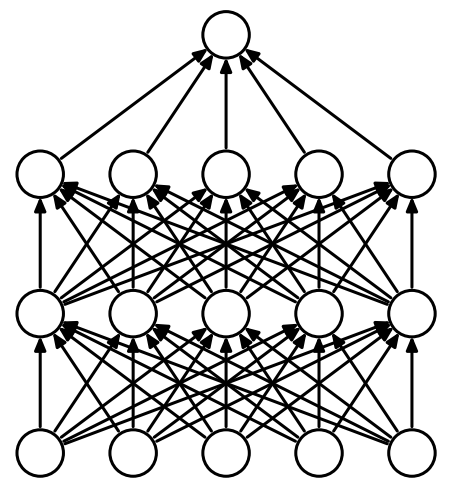
\includegraphics[height=0.4\textheight]{Figs/Dropout-before.png}
			\caption{Behavior of dropout at testing time. \href{https://www.cs.toronto.edu/~hinton/absps/JMLRdropout.pdf}{Source}}
		\end{figure}
	\end{block}
\end{frame}
\begin{frame}{Solution 3: Dropout}
	\begin{block}{Performance}
		\begin{itemize}
			\item the dependence between different neuron decreases
			\begin{itemize}
				\item neurons get more generalized
			\end{itemize}
		\end{itemize}
		
		\begin{figure}[H]
			\centering
			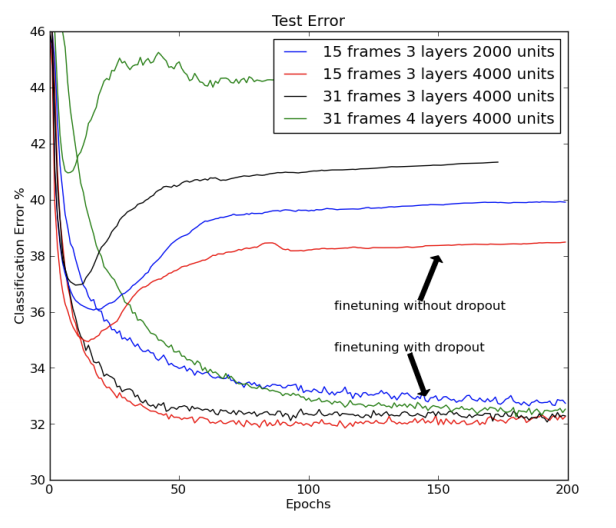
\includegraphics[height=0.4\textheight]{Figs/section_4/dropout_performance.png}
			\caption{the effect of dropout layer. as you see, the total error is reduced by a considerable amount. \href{https://towardsdatascience.com/understanding-and-implementing-dropout-in-tensorflow-and-keras-a8a3a02c1bfa}{Source}}
		\end{figure}
	\end{block}
\end{frame}
\begin{frame}{Solution 3: Dropout}
	\begin{block}{Practice tips}
		\begin{itemize}
			\item you can tweak dropout rate if you still see overfitting issues
			\begin{itemize}
				\item still overfitting -> increase dropout rate
				\item underfitting -> decrease dropout rate
			\end{itemize}
			\item layersize $\sim$ dropout rate
			\item usually in practice, people will use dropout after the last hidden layer
		\end{itemize}
	\end{block}
\end{frame}



\begin{frame}{Problem: Vanishing/Exploding Gradients}
	// Todo
    \begin{itemize}
    	\item beginning of learning -> He/ELU
    	\item during learning -> still exists
    \end{itemize}
    
    \begin{figure}[H]
    	\centering
    	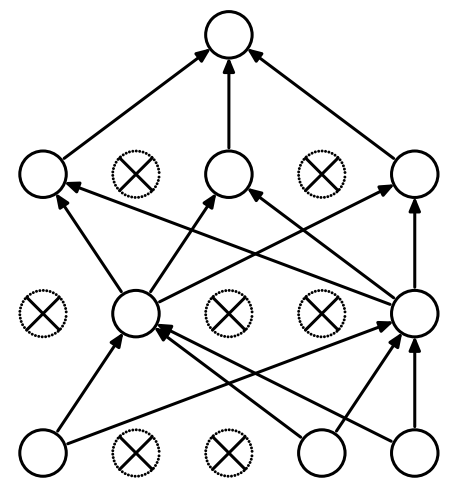
\includegraphics[height=0.4\textheight]{Figs/Dropout-after.png}
    	\caption{Behavior of dropout at training time. \href{https://www.cs.toronto.edu/~hinton/absps/JMLRdropout.pdf}{Source}}
    \end{figure}
\end{frame}

\begin{frame}{Solution: Batch Norm layer}
	\begin{itemize}
		\item for normalizing the data
	\end{itemize}
	\begin{figure}[H]
		\centering
		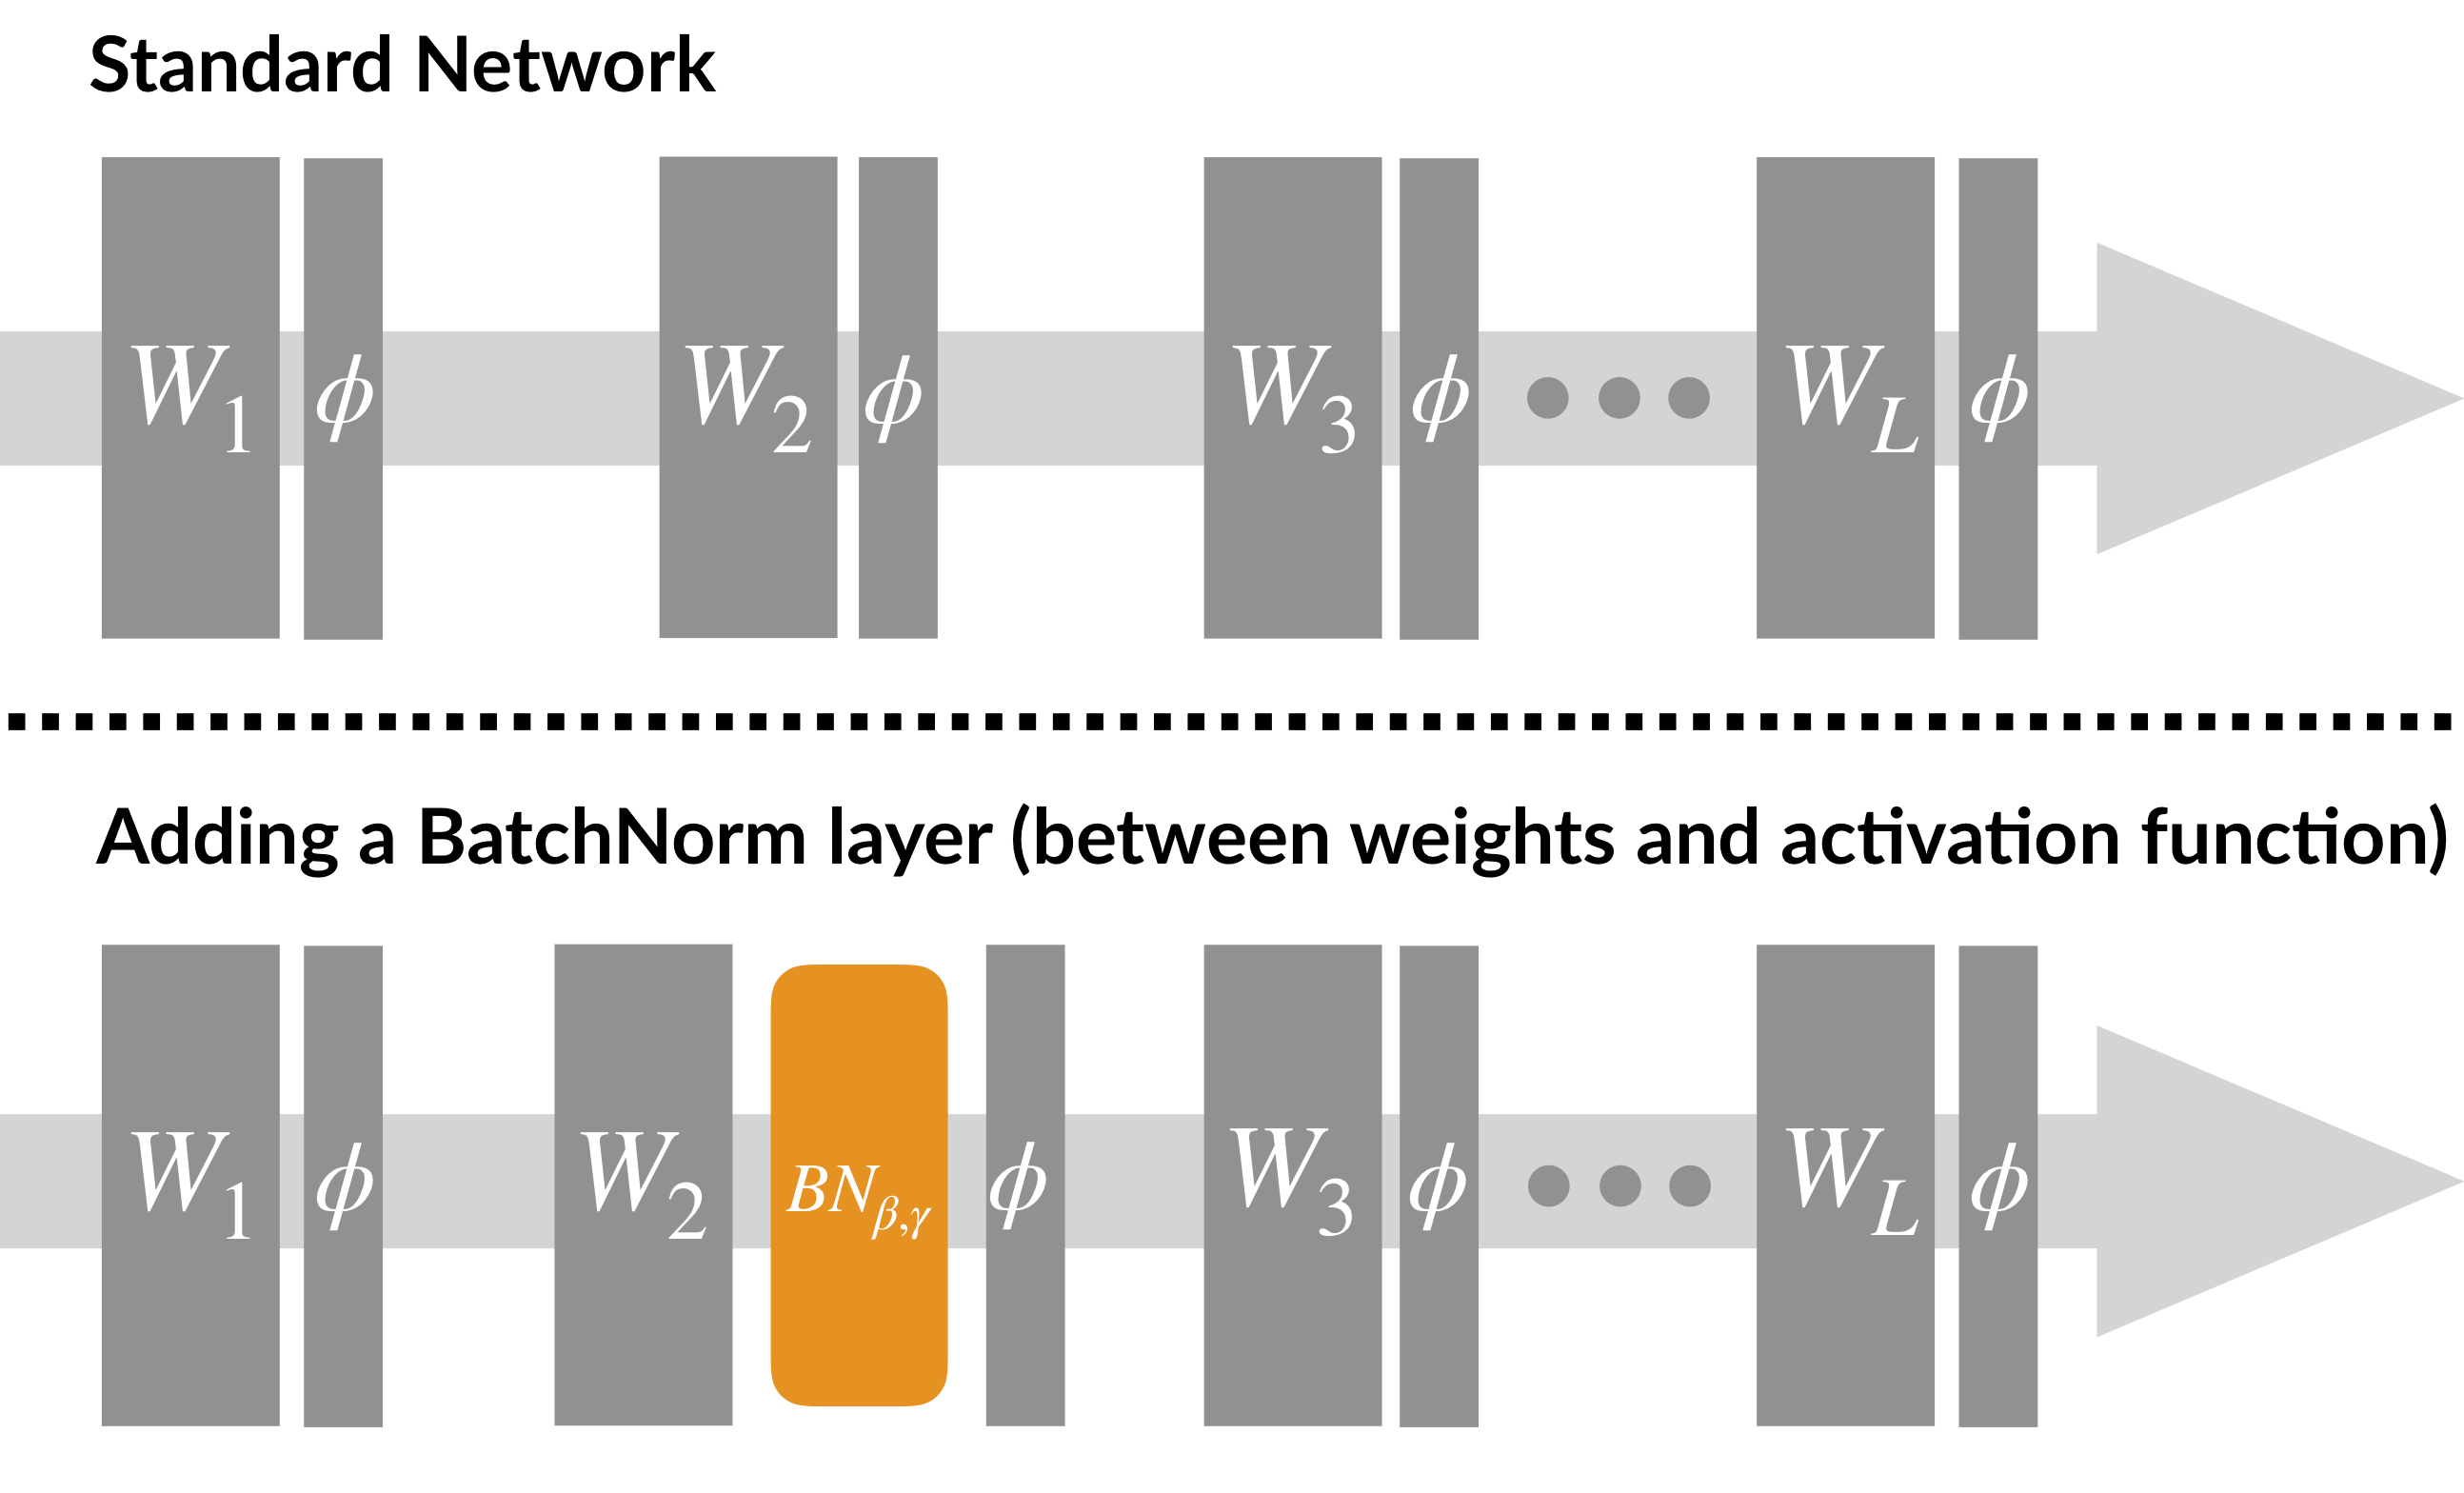
\includegraphics[width=0.75\textwidth]{Figs/section_4/batchnorm_2.jpg}
		\caption{where batchnorm layer is placed \href{https://gradientscience.org/batchnorm/}{source}}
	\end{figure}
\end{frame}
\begin{frame}{Solution: Batch Norm layer}
	\begin{block}{Training}
		\begin{itemize}
			\item zero-centers and normalizes a batch
		\end{itemize}
		\begin{equation*}
			\mathlarger{
				\mu_B := \frac{1}{N_B} \sum{x_B^{(i)}}
			}
		\end{equation*}
		\begin{equation*}
			\mathlarger{
				\sigma_B^2 := \frac{1}{N_B} \sum{(x_B^{(i)} - \mu_B)^2}
			}
		\end{equation*}
		\begin{equation*}
			\mathlarger{
				\hat{x_B}^{(i)} = \frac{x_B^{(i)} - \mu_B}{\sqrt{\sigma^2_B + \epsilon}}
			}
		\end{equation*}
		\begin{itemize}
			\item then, scales and shifts with two learnable parameters $\gamma, \beta$
		\end{itemize}
		\begin{equation*}
			\mathlarger{
				y_B^{(i)} = \gamma \hat{x_B}^{(i)} + \beta	
			}
		\end{equation*}
	\end{block}
\end{frame}
\begin{frame}{Solution: Batch Norm layer}
	\begin{block}{Testing}
		\begin{itemize}
			\item to zero-center and normalize the input, we need average and variance of the whole data
			\item that can be acquired during the learning
			\item therefore two more learnable parameters!
		\end{itemize}
		\vspace{0.1\textheight}
			\begin{equation}
				\mathlarger{
					\mu := \frac{1}{N} \sum{x^{(i)}}
				}
			\end{equation}
			\begin{equation}
				\mathlarger{
					\sigma^2 := \frac{1}{N} \sum{(x^{(i)} - \mu)^2}
				}
			\end{equation}
	\end{block}
\end{frame}
\begin{frame}{Solution: Batch Norm layer}
	\begin{block}{Performance}
		\begin{itemize}
			\item data gets normalized
			\begin{itemize}
				\item convergence improves
			\end{itemize}
		\end{itemize}
		\begin{figure}[H]
			\centering
			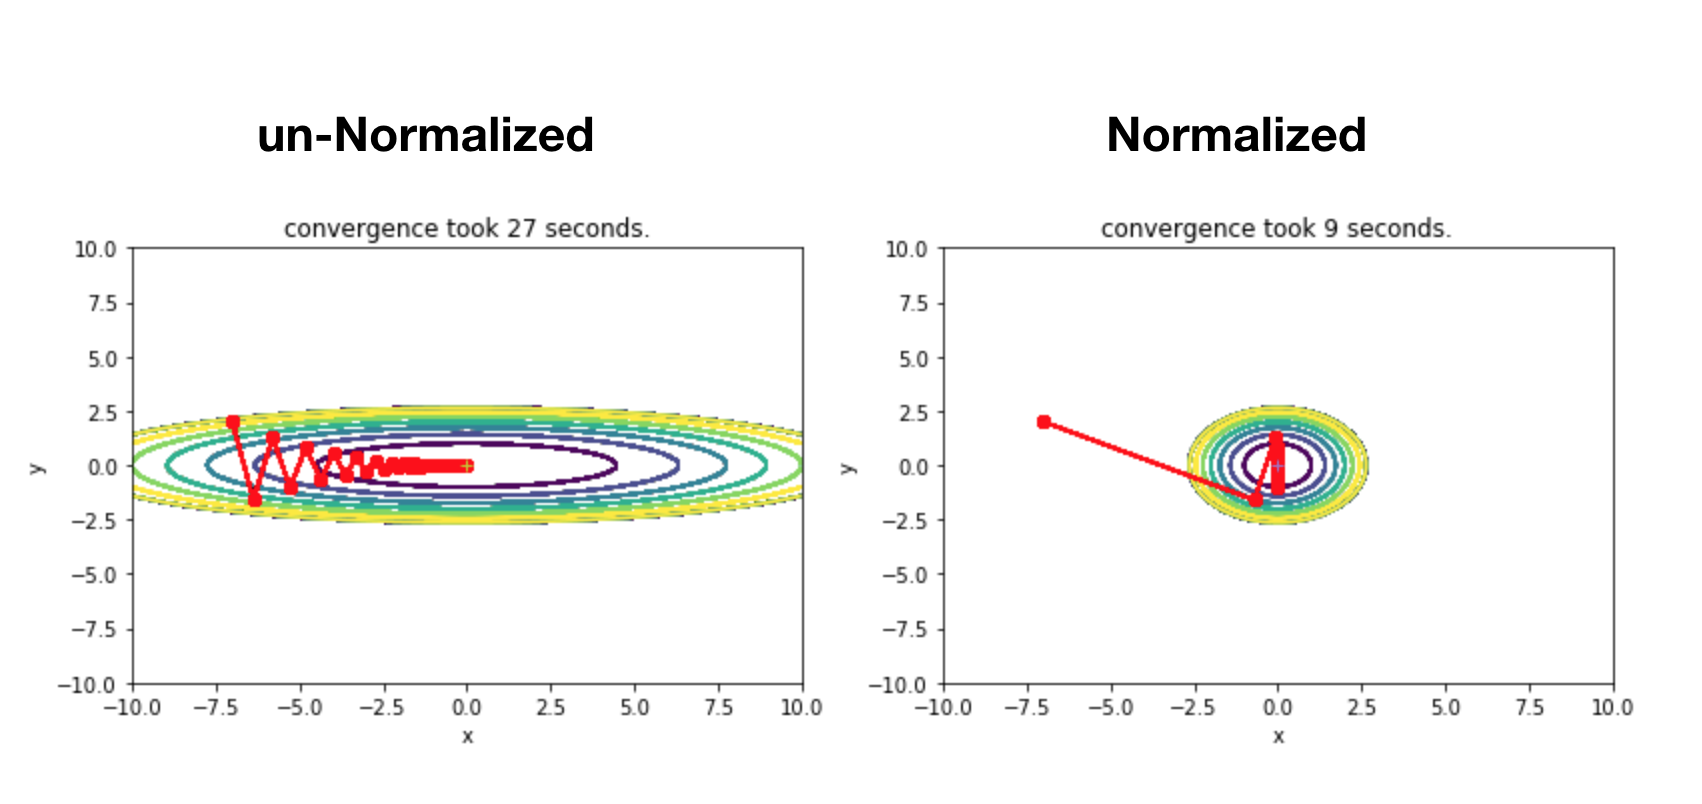
\includegraphics[width=0.75\textwidth]{Figs/section_4/batchnorm_3.png}
			\caption{batchnorm performance. as you see, convergence speed is increased by 200\% in this problem.  \href{https://jsideas.net/batch_normalization/}{source}}
		\end{figure}
	\end{block}
\end{frame}
\begin{frame}{Solution: Batch Norm layer}
	\begin{block}{Pros}
		\begin{itemize}
			\item vanishing gradient problem reduced
			\begin{itemize}
				\item can use even saturating activation functions (tanh, logistics, etc.)
			\end{itemize}
			\item much less sensitive to initial weight
			\item exploding gradient problem reduced
			\begin{itemize}
				\item being able to use longer learning rates , which speeds up learning
			\end{itemize}
			\item acts as a regularizer, too
			\begin{itemize}
				\item no need for other regularizer techniques (dropout, etc.)
			\end{itemize}
		\end{itemize}
	\end{block}
\end{frame}
\begin{frame}{Solution: Batch Norm layer}
	\begin{block}{Cons}
		\begin{itemize}
			\item adds complexity to the model (more parameters and computations)
			\begin{itemize}
				\item after training, we can mix the layer with its previous one
			\end{itemize}
		\end{itemize}
			\begin{equation}
				\mathlarger{x'^{(i)} = W x^{(i)} + b}
			\end{equation}
			\begin{equation}
				\mathlarger{y^{(i)} = \frac{x'^{(i)} - \mu}{\sqrt{\sigma^2 + \epsilon}} + \beta}
			\end{equation}
			\begin{equation}
				\mathlarger{y^{(i)} = W' x^{(i)} + b'}
			\end{equation}
			\begin{equation}
				\mathlarger{
					W' := \frac{1}{\sqrt{\sigma^2 + \epsilon}} W	
				}
			\end{equation}
			\begin{equation}
				\mathlarger{
					b' := \beta + \frac{b- \mu}{\sqrt{\sigma^2 + \epsilon}}	
				}
			\end{equation}
	\end{block}
\end{frame}
\begin{frame}{Solution: Batch Norm layer}
	Examples
	\begin{itemize}
		\item todo. examples from the book?
	\end{itemize}
\end{frame}